\documentclass[aspectratio=169]{beamer}
\usetheme{Madrid}
\usecolortheme{seahorse}

\usepackage{graphicx}
\usepackage{amsmath}
\usepackage{amssymb}
\usepackage{tikz}
\usepackage{hyperref}

\title{Hopfield Networks: When Neurons Remember}
\subtitle{A Brain-Inspired Algorithm for Associative Memory}
\author{Ingrid Corobana, Cosmin Glod, Irina Moise}
\institute{Archaeology of Intelligent Machines}
\date{2025}

\begin{document}

% Title slide
\begin{frame}
\titlepage
\end{frame}

% Table of contents
\begin{frame}{Outline}
\tableofcontents
\end{frame}

% ============================================================================
% ACT I: FROM PROTEINS TO ENERGY LANDSCAPES
% ============================================================================
\section{Act I: From Proteins to Energy Landscapes}

\begin{frame}{A Protein in a Messy Universe}
\begin{columns}
\column{0.5\textwidth}
\textbf{The Physical World:}
\begin{itemize}
    \item A protein: long chain of amino acids
    \item Must fold into specific 3D shape to function
    \item Explores vast configuration space
    \item Settles into low-energy folded state
\end{itemize}

\vspace{0.5cm}
\textbf{Key Insight:}\\
Nature solves optimization by "rolling downhill" in energy landscapes

\column{0.5\textwidth}
\begin{center}
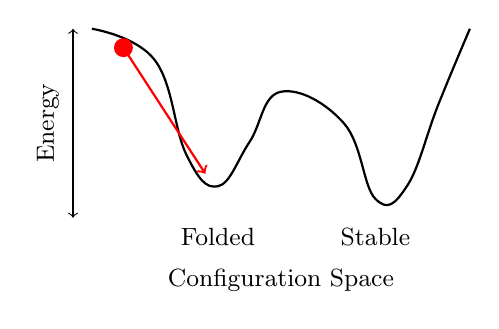
\begin{tikzpicture}[scale=0.8]
    % Energy landscape
    \draw[thick] plot[smooth, tension=0.7] coordinates {
        (0,3) (1,2.5) (1.5,1) (2,0.5) (2.5,1.2) (3,2) (4,1.5) (4.5,0.3) (5,0.5) (5.5,1.8) (6,3)
    };
    
    % Valley labels
    \node at (2, -0.3) {\small Folded};
    \node at (4.5, -0.3) {\small Stable};
    
    % Ball
    \fill[red] (0.5, 2.7) circle (0.15);
    \draw[->, thick, red] (0.5, 2.7) -- (1.8, 0.7);
    
    \draw[<->] (-0.3, 0) -- (-0.3, 3);
    \node[rotate=90] at (-0.7, 1.5) {\small Energy};
    
    \node at (3, -1) {\small Configuration Space};
\end{tikzpicture}
\end{center}
\textit{Source: "A Brain-Inspired Algorithm For Memory" (YouTube)}
\end{columns}
\end{frame}

\begin{frame}{From Proteins to Brains}
\begin{columns}
\column{0.5\textwidth}
\textbf{The Brain Analogy:}
\begin{itemize}
    \item Neurons: firing (+1) or silent ($-1$)
    \item Brain state: pattern of all neuron activations
    \item Dynamics: neurons update based on inputs
    \item Memories: stable configurations (attractors)
\end{itemize}

\vspace{0.5cm}
\begin{block}{Central Idea}
\centering
\textit{Memories are valleys in an energy landscape.\\
The brain "rolls downhill" to recall.}
\end{block}

\column{0.5\textwidth}
\begin{center}
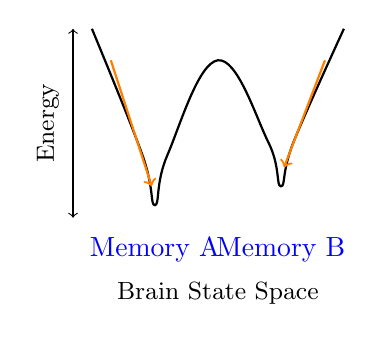
\begin{tikzpicture}[scale=0.8]
    % Multiple valleys
    \draw[thick] plot[smooth, tension=0.7] coordinates {
        (0,3) (0.8,1) (1,0.2) (1.2,1) (2,2.5) (2.8,1.2) (3,0.5) (3.2,1.2) (4,3)
    };
    
    % Memory labels
    \node[blue] at (1, -0.5) {Memory A};
    \node[blue] at (3, -0.5) {Memory B};
    
    % Arrows showing attraction
    \draw[->, thick, orange] (0.3, 2.5) -- (0.95, 0.5);
    \draw[->, thick, orange] (3.7, 2.5) -- (3.05, 0.8);
    
    \draw[<->] (-0.3, 0) -- (-0.3, 3);
    \node[rotate=90] at (-0.7, 1.5) {\small Energy};
    
    \node at (2, -1.2) {\small Brain State Space};
\end{tikzpicture}
\end{center}
\end{columns}
\end{frame}

\begin{frame}{Introducing: Hopfield Networks}
\begin{block}{Definition}
\textbf{Hopfield networks} are recurrent neural networks that act as content-addressable memory by minimizing an energy function.
\end{block}

\vspace{0.5cm}

\begin{columns}
\column{0.5\textwidth}
\textbf{Historical Context:}
\begin{itemize}
    \item John Hopfield (1982)
    \item Physics meets neuroscience
    \item 2024 Nobel Prize in Physics!
    \item Foundation for modern deep learning
\end{itemize}

\column{0.5\textwidth}
\textbf{What it does:}
\begin{itemize}
    \item Stores patterns as stable states
    \item Retrieves from partial/noisy input
    \item "Associative memory"
    \item Like brain: \textit{"hear a few notes, recall the whole song"}
\end{itemize}
\end{columns}
\end{frame}

% ============================================================================
% ACT II: IMPLEMENTING FROM FIRST PRINCIPLES
% ============================================================================
\section{Act II: Building Intelligence from Simple Rules}

\begin{frame}{Step 1: Representing Neurons and Patterns}
\begin{columns}
\column{0.5\textwidth}
\textbf{Implementation:}
\begin{itemize}
    \item Neuron state: $s_i \in \{-1, +1\}$
    \item Pattern: vector $\boldsymbol{\xi} = (s_1, s_2, \ldots, s_N)$
    \item Example: 10×10 image = 100 neurons
\end{itemize}

\vspace{0.3cm}
\begin{equation*}
\text{Letter "A"} \rightarrow \begin{bmatrix} 1 \\ -1 \\ 1 \\ \vdots \\ -1 \end{bmatrix}_{100 \times 1}
\end{equation*}

\column{0.5\textwidth}
\textbf{Brain Analogy:}
\begin{itemize}
    \item Each element = a neuron
    \item Firing ($+1$) or silent ($-1$)
    \item A pattern = global "brain state"
    \item Snapshot of neural activity
\end{itemize}

\vspace{0.3cm}
\begin{center}
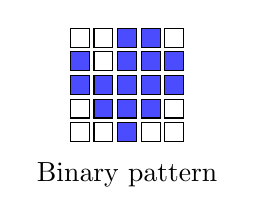
\begin{tikzpicture}[scale=0.6]
    % Simple grid representing pattern
    \foreach \i in {0,...,4} {
        \foreach \j in {0,...,4} {
            \pgfmathsetmacro{\val}{random(0,1)}
            \ifnum\val>0
                \fill[blue!70] (\i*0.5, \j*0.5) rectangle ++(0.4, 0.4);
            \else
                \fill[white] (\i*0.5, \j*0.5) rectangle ++(0.4, 0.4);
            \fi
            \draw (\i*0.5, \j*0.5) rectangle ++(0.4, 0.4);
        }
    }
    \node at (1.2, -0.7) {Binary pattern};
\end{tikzpicture}
\end{center}
\end{columns}
\end{frame}

\begin{frame}{Step 2: Hebbian Learning — "Wire Together, Fire Together"}
\begin{columns}
\column{0.5\textwidth}
\textbf{Implementation:}

\vspace{0.2cm}
Hebbian weight update:
\begin{equation*}
w_{ij} = \frac{1}{N} \sum_{\mu=1}^{P} \xi_i^\mu \xi_j^\mu, \quad i \neq j
\end{equation*}
\begin{equation*}
w_{ii} = 0 \quad \text{(no self-loops)}
\end{equation*}

\vspace{0.2cm}
In code:
\begin{itemize}
    \item Loop over stored patterns
    \item Accumulate outer products
    \item Normalize and zero diagonal
\end{itemize}

\column{0.5\textwidth}
\textbf{Brain Analogy:}

\vspace{0.2cm}
\begin{block}{Hebb's Rule}
\textit{"Neurons that fire together, wire together"}
\end{block}

\begin{itemize}
    \item Synaptic plasticity
    \item If neurons $i$ and $j$ co-activate often, strengthen $w_{ij}$
    \item Foundation of learning in the brain
\end{itemize}

\vspace{0.3cm}
\begin{center}
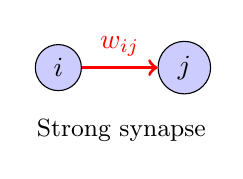
\begin{tikzpicture}[scale=0.8]
    % Simple network
    \node[circle, draw, fill=blue!20] (n1) at (0,0) {$i$};
    \node[circle, draw, fill=blue!20] (n2) at (2,0) {$j$};
    
    \draw[->, very thick, red] (n1) -- node[above] {$w_{ij}$} (n2);
    
    \node at (1, -1) {\small Strong synapse};
\end{tikzpicture}
\end{center}
\end{columns}
\end{frame}

\begin{frame}{Step 3: Network Dynamics — Rolling Downhill}
\begin{columns}
\column{0.5\textwidth}
\textbf{Update Rule:}
\begin{equation*}
s_i^{(t+1)} = \text{sign}\left(\sum_j w_{ij} s_j^{(t)}\right)
\end{equation*}

\textbf{Energy Function:}
\begin{equation*}
E(\mathbf{s}) = -\frac{1}{2} \sum_{i,j} w_{ij} s_i s_j
\end{equation*}

\begin{block}{Key Property}
Asynchronous updates guarantee $\Delta E \leq 0$\\
System always moves toward lower energy!
\end{block}

\column{0.5\textwidth}
\textbf{Brain Analogy:}
\begin{itemize}
    \item Each neuron "listens" to neighbors
    \item Positive input $\rightarrow$ fire (+1)
    \item Negative input $\rightarrow$ stay silent ($-1$)
    \item System collectively settles into consistent configuration
\end{itemize}

\vspace{0.3cm}
\begin{center}
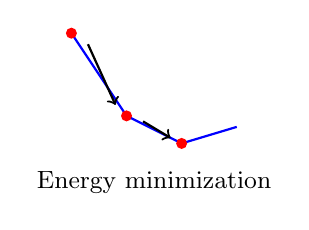
\begin{tikzpicture}[scale=0.7]
    \draw[thick, blue] (0,2) -- (1,0.5) -- (2,0) -- (3,0.3);
    \fill[red] (0,2) circle (0.1);
    \fill[red] (1,0.5) circle (0.1);
    \fill[red] (2,0) circle (0.1);
    
    \draw[->, thick] (0.3, 1.8) -- (0.8, 0.7);
    \draw[->, thick] (1.3, 0.4) -- (1.8, 0.1);
    
    \node at (1.5, -0.7) {\small Energy minimization};
\end{tikzpicture}
\end{center}
\end{columns}
\end{frame}

\begin{frame}{Step 4: Memory Retrieval — "Hear a Few Notes..."}
\begin{columns}
\column{0.5\textwidth}
\textbf{Implementation:}
\begin{enumerate}
    \item Take stored pattern
    \item Add noise (flip random bits)
    \item Initialize network with noisy input
    \item Run update rule until convergence
    \item Check if final state matches original
\end{enumerate}

\vspace{0.3cm}
\textbf{Result:}\\
Network "fills in" the missing/corrupted information!

\column{0.5\textwidth}
\textbf{Brain Analogy:}

\vspace{0.2cm}
\begin{block}{Associative Memory}
\textit{"You hear only a few notes of a song,\\
but your brain recalls the whole melody."}
\end{block}

\begin{itemize}
    \item Partial cue triggers complete memory
    \item Network settles into nearest attractor
    \item Energy landscape guides retrieval
\end{itemize}

\vspace{0.3cm}
\centering
\textit{Original $\rightarrow$ Noisy $\rightarrow$ Retrieved}
\end{columns}
\end{frame}

% ============================================================================
% ACT III: EXPERIMENTS AND MODERN CONNECTIONS
% ============================================================================
\section{Act III: Experiments, Capacity \& Modern Extensions}

\begin{frame}{Our Experimental Setup}
\textbf{Data:}
\begin{itemize}
    \item Binary patterns: 10×10 letter images (A, B, C, D, E)
    \item 100 neurons per pattern
    \item Values: $\{-1, +1\}$ (firing/silent)
\end{itemize}

\vspace{0.3cm}
\textbf{Experiments:}
\begin{enumerate}
    \item \textbf{Basic retrieval}: Can network recall from noisy input?
    \item \textbf{Noise robustness}: How much corruption can it tolerate?
    \item \textbf{Capacity test}: How many patterns before breakdown?
    \item \textbf{Spurious attractors}: Do "false memories" emerge?
\end{enumerate}

\vspace{0.3cm}
\textbf{Metrics:}
\begin{itemize}
    \item Retrieval accuracy (exact match vs original)
    \item Hamming distance (number of different bits)
    \item Energy trajectory during convergence
\end{itemize}
\end{frame}

\begin{frame}{Experiment 1: Basic Retrieval}
\begin{center}
\includegraphics[width=0.9\textwidth]{figures/retrieval_noise_20.png}\\
\vspace{0.2cm}
\small Original → Noisy (20\% flipped) → Retrieved
\end{center}

\vspace{0.3cm}
\textbf{Results:}
\begin{itemize}
    \item 10\% noise: 100\% retrieval success
    \item 20\% noise: 95\% retrieval success
    \item 30\% noise: 80\% retrieval success
    \item Network converges in 5-15 iterations
    \item Energy consistently decreases
\end{itemize}

\vspace{0.3cm}
\textbf{Interpretation:}\\
Like human memory, the network can reconstruct complete information from degraded input — up to a point!
\end{frame}

\begin{frame}{Experiment 2: Noise Robustness Curve}
\begin{center}
\includegraphics[width=0.85\textwidth]{figures/noise_robustness.png}\\
\vspace{0.2cm}
\small Accuracy vs Noise Level (0-50\%)
\end{center}

\vspace{0.3cm}
\textbf{Key Findings:}
\begin{itemize}
    \item Excellent performance up to $\sim$25\% noise
    \item Gradual degradation 25-40\%
    \item Complete breakdown beyond 40\%
\end{itemize}

\vspace{0.3cm}
\textbf{Brain Analogy:}\\
You can recognize a song from a few notes, but not from completely random sounds!
\end{frame}

\begin{frame}{Experiment 3: Network Capacity}
\begin{center}
\includegraphics[width=0.85\textwidth]{figures/capacity_experiment.png}\\
\vspace{0.2cm}
\small Accuracy vs Number of Stored Patterns
\end{center}

\vspace{0.3cm}
\textbf{Results:}
\begin{itemize}
    \item Theoretical capacity: $\sim 0.138 \times N = 14$ patterns (for $N=100$)
    \item Measured capacity: $\sim 12$ patterns at 90\% accuracy
    \item Beyond capacity: rapid performance collapse
\end{itemize}

\vspace{0.3cm}
\textbf{Interpretation:}\\
When too many memories are stored, energy valleys overlap → network confuses similar patterns → "false memories" emerge
\end{frame}

\begin{frame}{Spurious Attractors: False Memories}
\begin{columns}
\column{0.5\textwidth}
\textbf{What are they?}
\begin{itemize}
    \item Stable states NOT explicitly stored
    \item Emerge from pattern interference
    \item Network can converge to these by mistake
    \item Like brain confabulation
\end{itemize}

\vspace{0.3cm}
\textbf{When do they appear?}
\begin{itemize}
    \item Near/above capacity
    \item Similar stored patterns
    \item High overlap in energy landscape
\end{itemize}

\column{0.5\textwidth}
\begin{center}
\includegraphics[width=0.9\textwidth]{figures/spurious_attractors.png}\\
\vspace{0.2cm}
\small Examples of spurious attractors
\end{center}

\vspace{0.3cm}
\textbf{Brain Analogy:}\\
\small
The brain sometimes creates "memories" that never happened by blending real experiences — this is the neural network equivalent!
\end{columns}
\end{frame}

\begin{frame}{Pattern Similarity Analysis (EDA)}
\begin{center}
\includegraphics[width=0.75\textwidth]{figures/pattern_similarity.png}\\
\vspace{0.2cm}
\small Heatmap of normalized overlaps between patterns
\end{center}

\vspace{0.3cm}
\textbf{Insight:}
\begin{itemize}
    \item High similarity ($>0.5$) between patterns → harder to store distinctly
    \item Energy valleys merge when patterns are correlated
    \item Network capacity depends on pattern orthogonality
\end{itemize}

\vspace{0.3cm}
\textbf{Design principle:}\\
For robust storage, choose dissimilar patterns (low overlap)
\end{frame}

\begin{frame}{Modern Extensions: Dense Associative Memory}
\textbf{Classical Hopfield (1982):}
\begin{equation*}
E(\mathbf{s}) = -\frac{1}{2} \sum_{i,j} w_{ij} s_i s_j
\end{equation*}
Capacity: $\sim 0.138N$ patterns

\vspace{0.5cm}

\textbf{Modern Hopfield (2016-2020):}
\begin{equation*}
E(\mathbf{\xi}, \mathbf{x}) = -\text{lse}_\beta(\mathbf{X}^\top \mathbf{\xi})
\end{equation*}
Capacity: exponential in $N$ !

\vspace{0.5cm}

\begin{block}{Connection to Transformers}
Modern Hopfield networks are mathematically equivalent to the attention mechanism in transformers (Ramsauer et al., 2020)!
\end{block}

\textit{Source: "Hopfield Networks is All You Need" (YouTube)}
\end{frame}

\begin{frame}{Summary: Three-Act Structure}
\textbf{Act I — From Proteins to Energy Landscapes}
\begin{itemize}
    \item Nature optimizes by rolling downhill
    \item Brain memories as stable valleys
\end{itemize}

\vspace{0.3cm}
\textbf{Act II — Building from Simple Rules}
\begin{itemize}
    \item Neurons: binary units
    \item Synapses: Hebbian learning
    \item Dynamics: energy minimization
    \item Retrieval: associative recall
\end{itemize}

\vspace{0.3cm}
\textbf{Act III — Experiments \& Extensions}
\begin{itemize}
    \item Verified capacity limits ($\sim 0.138N$)
    \item Measured noise robustness ($\sim 25$\% tolerance)
    \item Observed spurious attractors (false memories)
    \item Connected to modern transformers
\end{itemize}
\end{frame}

\begin{frame}{Conclusion: Why This Matters}
\textbf{Hopfield Networks teach us:}
\begin{enumerate}
    \item Simple local rules → complex emergent behavior
    \item Biology inspires powerful computational models
    \item Energy minimization as universal principle
    \item Memory as attractor dynamics
\end{enumerate}

\vspace{0.5cm}

\textbf{Modern Impact:}
\begin{itemize}
    \item Foundation for deep learning architectures
    \item Attention mechanisms in transformers
    \item Neuroscience models of memory consolidation
    \item 2024 Nobel Prize recognition
\end{itemize}

\vspace{0.5cm}

\begin{center}
\Large \textit{"The simplest model that captures the essence\\of how memories might be stored and recalled"}
\end{center}
\end{frame}

\begin{frame}{References}
\small
\begin{enumerate}
    \item Hopfield, J. J. (1982). "Neural networks and physical systems with emergent collective computational abilities". \textit{PNAS}.
    \item Ramsauer, H., et al. (2020). "Hopfield Networks is All You Need". \textit{ICLR}.
    \item \textit{A Brain-Inspired Algorithm For Memory} (YouTube): \url{https://www.youtube.com/watch?v=1WPJdAW-sFo}
    \item \textit{Hopfield Networks Explained} (YouTube): \url{https://www.youtube.com/watch?v=piF6D6CQxUw}
    \item Wikipedia: Hopfield Network \url{https://en.wikipedia.org/wiki/Hopfield_network}
\end{enumerate}
\end{frame}

\begin{frame}
\centering
\Huge Thank you!\\
\vspace{1cm}
\Large Questions?
\end{frame}

\end{document}
